\chapter{Épilogue}\label{ch:conclusion}
\setlength{\epigraphwidth}{0.90\textwidth}
\epigraph{``Nous sommes tous façonnés par les outils que nous utilisons, en particulier : les formalismes que nous utilisons façonnent nos habitudes de pensée, pour le meilleur ou pour le pire, et cela signifie que nous devons être très prudents dans le choix de ce que nous apprenons et enseignons, car le désapprentissage n'est pas vraiment possible.''}{\begin{flushright}--Edsger W. \citet{dijkstra2000answers}, \href{https://www.cs.utexas.edu/~EWD/transcriptions/EWD13xx/EWD1305.html}{\textit{Réponses aux questions des étudiants en génie logiciel}}\end{flushright}}

Dans cette thèse, nous avons exploré quatre outils de programmation différents issus du génie logiciel pour le développement de systèmes intelligents, en abordant de manière générale la complexité cognitive apparaissant dans les quatre phases de la méthode de la cascade de Royce. Ces outils ont des degrés variables de praticabilité, allant de très théoriques (par exemple l'essai contradictoire de programmes différentiables ~\autoref{ch:difftest}) à plus pragmatiques (par exemple la conteneurisation ~\autoref{ch:ducker}). Dans chaque chapitre, nous fournissons quelques exemples motivants qui démontrent les principales lacunes des outils de programmation de pointe pour les systèmes intelligents et nous proposons des solutions viables qui remédient à quelques-unes de ces lacunes. Bien que nous espérions que les programmeurs de systèmes intelligents (par exemple les roboticiens et les praticiens de l'apprentissage automatique) puissent tirer une certaine valeur des outils eux-mêmes, notre intention est d'être \textit{illustratif} plutôt que \textit{prescriptif}.

En construisant des outils et en validant leur efficacité sur des applications de jouets, nous espérons que les développeurs d'outils examineront attentivement comment les outils logiciels peuvent introduire et atténuer la complexité cognitive. Des outils bien conçus peuvent augmenter la capacité cognitive des humains à raisonner sur des faits en présence d'incertitude~\citep{famelis2012partial}, et fournir une assistance ergonomique de débogage et de visualisation (par exemple \autoref{ch:hatchery}). Nous espérons également faire comprendre l'importance de la conception notationnelle. Une bonne notation oblige les auteurs à réfléchir soigneusement à leurs abstractions, fait ressortir les erreurs logiques et les aide à comprendre les implications des premiers choix de conception. Nous espérons que les outils de programmation présentés dans cette thèse inciteront les développeurs à réimaginer le potentiel de la programmation assistée par ordinateur dans la conception de logiciels pour les systèmes intelligents.

En complétant les capacités cognitives des programmeurs humains -- qui excellent dans la résolution créative de problèmes et le raisonnement abstrait de haut niveau -- avec les capacités de traitement symbolique brut des outils de programmation, nous pouvons accélérer la conception~(\autoref{ch:hatchery}), le développement~(\autoref{ch:kotlingrad}), la validation~(\autoref{ch:difftest}) et le déploiement~(\autoref{ch:ducker}) de systèmes intelligents dans des applications du monde réel. Ce processus est un cycle vertueux qui mérite des outils et des pratiques spécifiques à chaque domaine en raison des possibilités offertes par les systèmes intelligents et de l'interaction unique entre l'intelligence humaine et l'intelligence des machines. Alors que nous commençons à développer des systèmes autonomes qui jouent un rôle de plus en plus actif dans la société, tant les ingénieurs en logiciel que les praticiens de l'apprentissage automatique doivent jouer un rôle tout aussi actif dans le façonnage du comportement de ces systèmes.

Les ingénieurs en logiciel ont un certain nombre de leçons à tirer des systèmes intelligents. Les concepteurs de langage feraient bien de considérer la valeur des outils de développement intelligents (\autoref{ch:hatchery}) pour faciliter le dialogue entre l'intelligence humaine et l'intelligence des machines. Les langages devraient s'efforcer d'intégrer les connaissances humaines par le biais de systèmes de programmation et de systèmes experts différentiables, afin d'aider à raisonner sur la composition et la justesse de la description (\autoref{ch:kotlingrad}). Des tests automatisés via des simulateurs et des cadres de tests de propriétés sont nécessaires pour raisonner sur l'exactitude opérationnelle sans spécification exhaustive (\autoref{ch:difftest}). Enfin, l'intégration continue, les tests automatisés et les meilleures pratiques dans les opérations des développeurs (\autoref{ch:ducker}) sont nécessaires pour garantir la reproductibilité des artefacts en présence de variabilité logicielle et matérielle.

Les praticiens de l'apprentissage automatique ont également un certain nombre de leçons à tirer du génie logiciel. Le génie logiciel traditionnel prescrit un modèle de processus et une méthodologie de test rigoureux qui ont guidé de nombreuses générations de projets logiciels. Pour devenir une véritable discipline d'ingénierie, l'apprentissage automatique devra adopter une approche plus systématique de la construction de systèmes autonomes. Les modèles d'apprentissage automatique sont formés sur des \textit{fonctions-objectives}, qui sont généralement des fonctions à faible dimension mesurant les performances d'un système et renvoyant une valeur scalaire connue sous le nom de \textit{erreur} ou \textit{perte}. En pratique, les systèmes intelligents doivent satisfaire à un ensemble de critères multiobjectifs~\citep{censi2015mathematical}, notamment l'efficacité énergétique~\citep{paull2010novel}, la mémoire~\citep{memory2013mitliagkas}, re/usability~\citep{breuleux2017automatic,deleu2019torchmeta}, predictability~\citep{turner2017well}, latency~\citep{ravanelli2018twin}, robustness~\citep{pineau2003policy}, reproductibilité~\citep{pineau2019improving}, explicabilité~\citep{turner2016model}, traçabilité~\citep{guo2017semantically, tsirigotis2018orion}, incertitude~\citep{diaz2018interactive}, simplicité~\citep{kastner2019representation}, fiabilité~\citep{xu2017efficient}, transférabilité~\citep{mehta2019active}, évolutivité~\citep{luan2019break} et bien d'autres facteurs.

Dans le domaine du génie logiciel traditionnel, il est raisonnable de supposer que ceux qui mettent en œuvre un nouveau système ont une certaine connaissance implicite du domaine et sont des êtres humains bien intentionnés travaillant à un objectif commun. Si on leur donne une description grossière, ils peuvent remplir les blancs. Lors de la construction d'un système intelligent, il serait plus sûr de supposer que les exigences sont mises en œuvre par un génie. Compte tenu de certaines données et d'une métrique d'optimisation, il faudra prendre tous les raccourcis possibles pour exaucer nos souhaits. Si nous ne prenons pas soin d'énoncer nos exigences, cette entité produira une solution qui ne fonctionne tout simplement pas (dans le meilleur des cas), ou qui semble fonctionner mais qui est vraiment maudite~\citep{bellman1957dynamic}.

Lors de la construction d'un système intelligent, les développeurs doivent soigneusement se demander : "Quel est le comportement souhaité du système que nous concevons? Cette question est souvent très gênante, car nos exigences approximatives doivent être traduites en contraintes précises sur l'espace de la solution. Par exemple, lors de la conception d'un véhicule autotracté, nous devons clairement optimiser la sécurité des passagers, mais en faisant cela, nous formerons un véhicule qui ne bouge jamais ou qui cède toujours aux véhicules qui passent. À défaut d'une spécification exhaustive, comment pouvons-nous être sûrs que le système qui en résultera répondra à nos exigences? La plupart des êtres humains sont capables de conduire un véhicule en toute sécurité, mais même les meilleurs ingénieurs ont du mal à écrire un algorithme de conduite. L'étiquetage des données à la main est trop coûteux. La vérification formelle est tout simplement impossible.

\begin{figure}
    \centering
    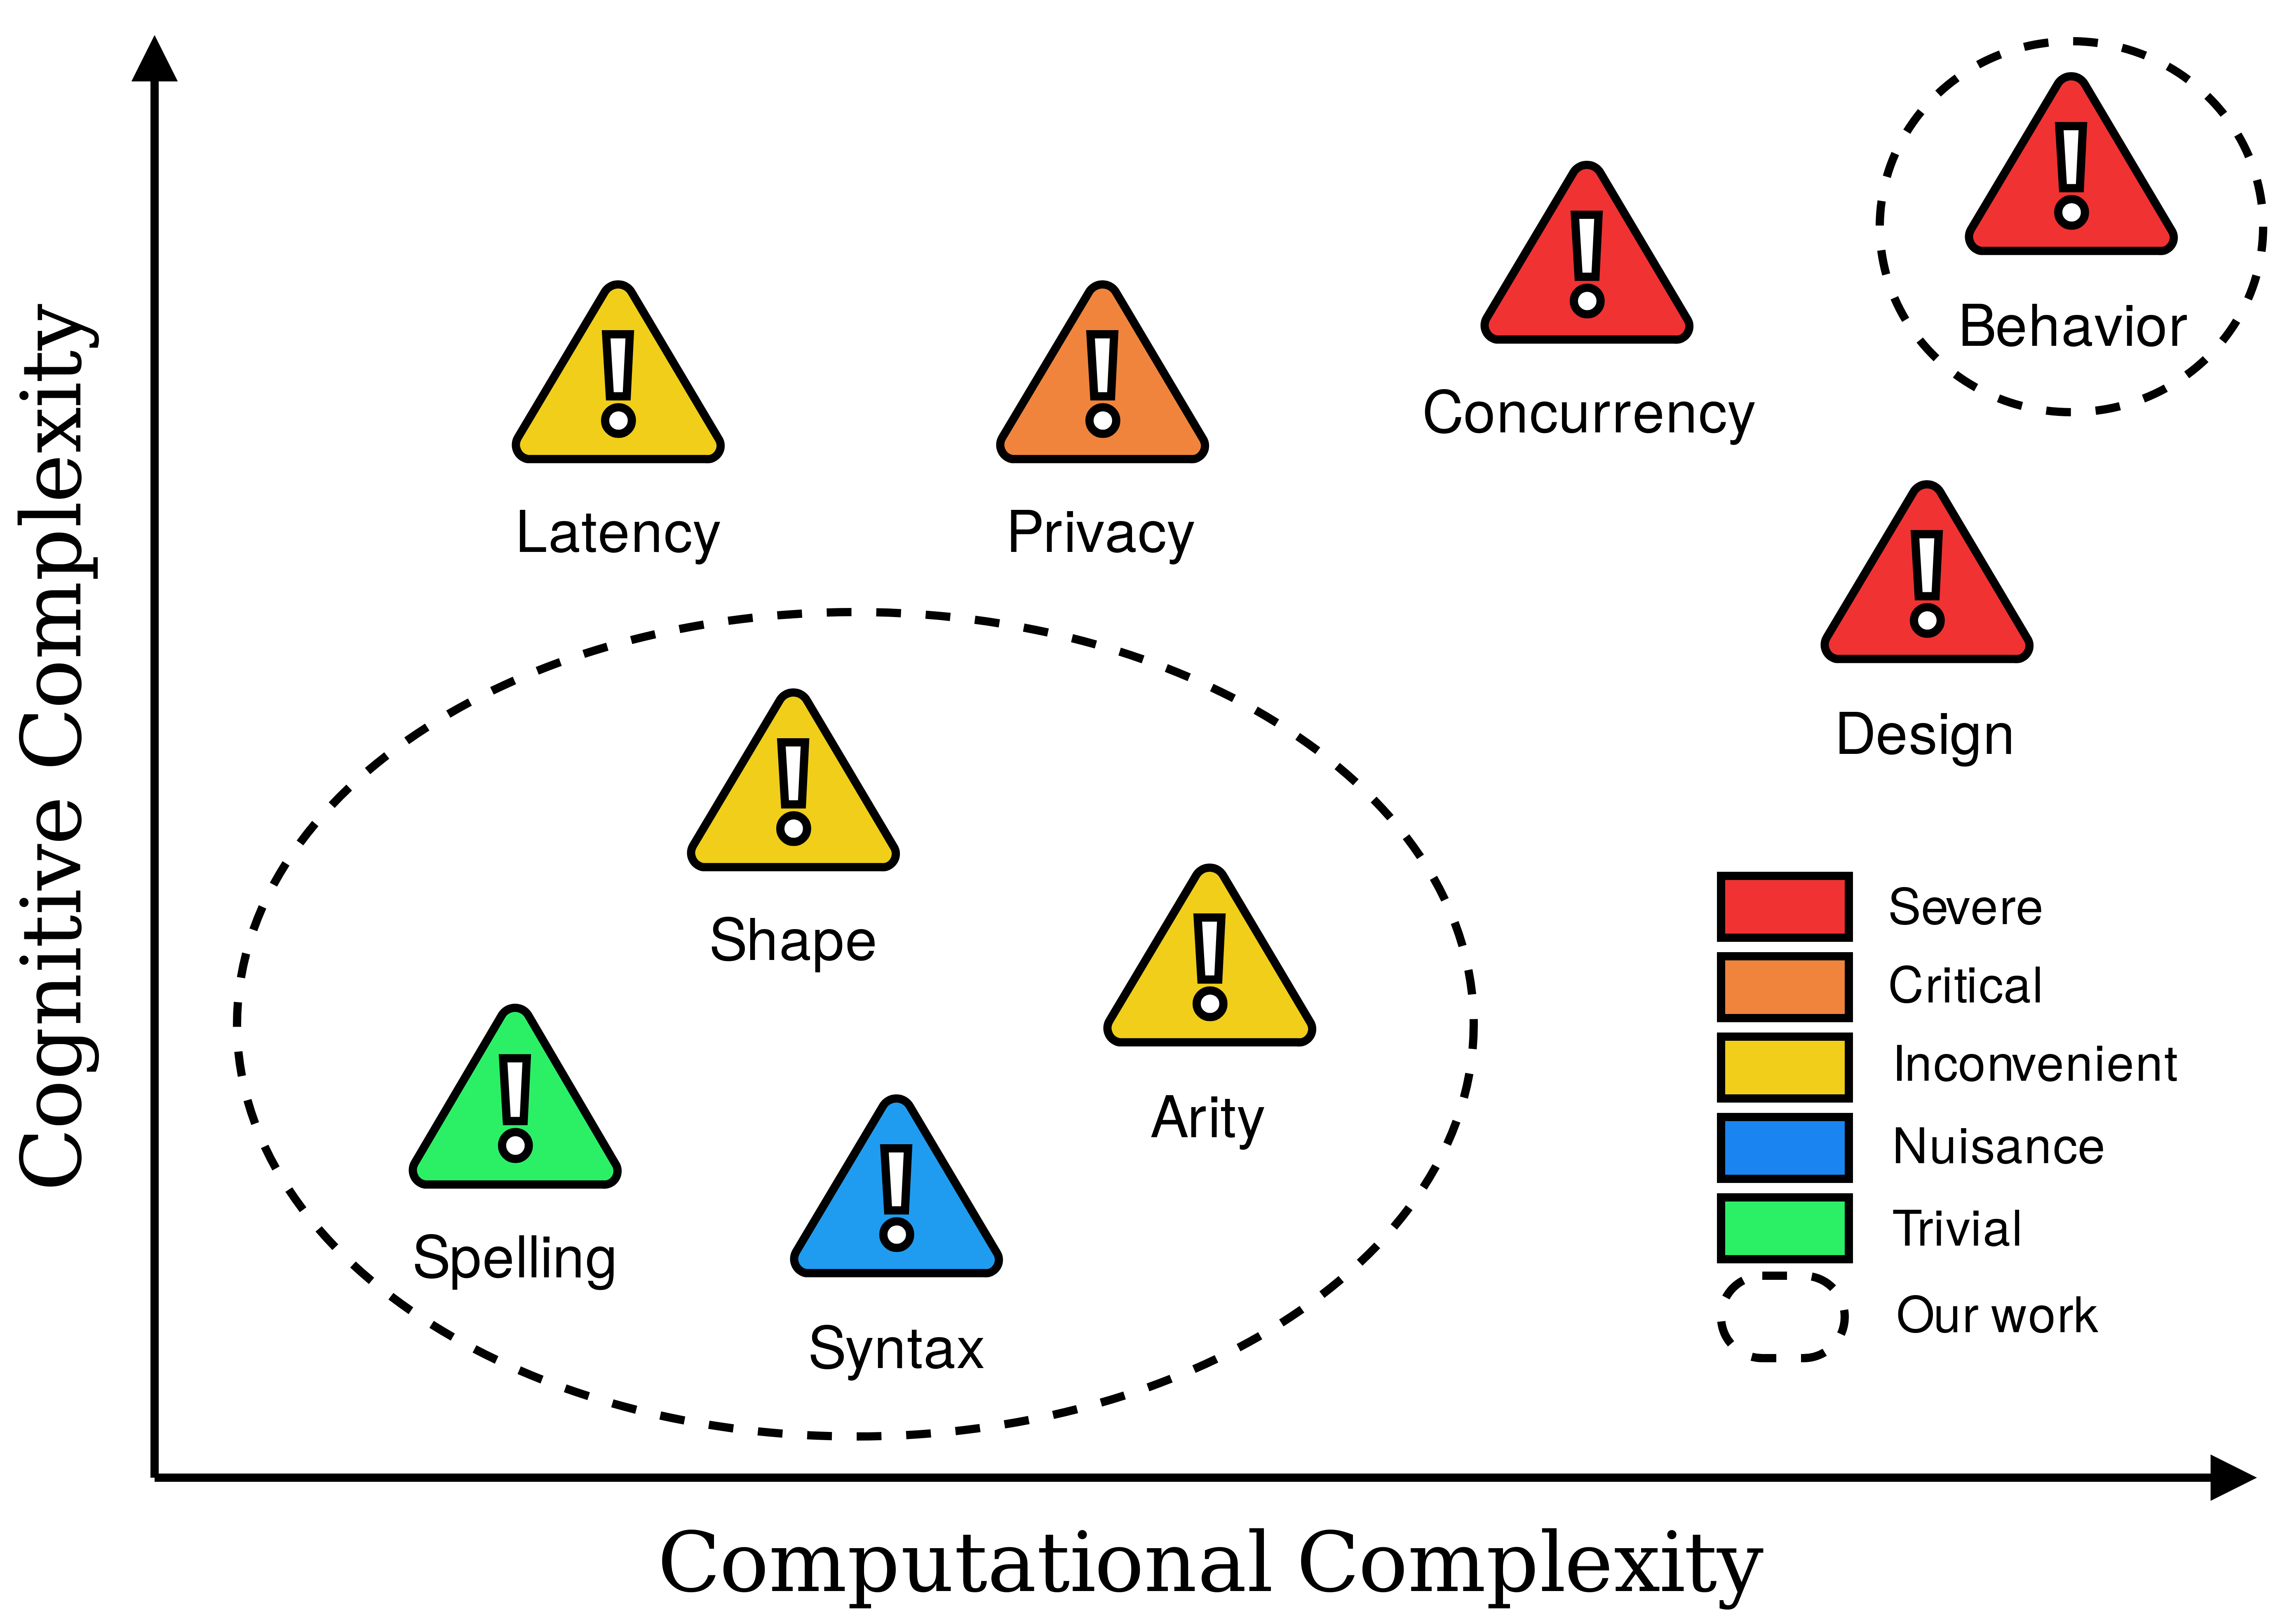
\includegraphics[width=0.60\textwidth]{../figures/verification_complexity.png}
    \caption{Complexité de la détection de divers types d'erreurs de programmation.}
    \label{fig:verification_complexity}
\end{figure}

Les systèmes de types, les compilateurs et les fuzzers font tous partie d'une catégorie plus large d'outils de validation et de vérification. L'objectif de ces outils est d'échanger la complexité cognitive contre la complexité informatique. Certaines erreurs (par exemple, les erreurs syntaxiques), sont des nuisances mineures et peuvent être détectées avec un bon analyseur incrémental (\autoref{subsec:the-parser}). D'autres, comme indiqué dans~\autoref{fig:verification_complexity}, présentent une complexité cognitive plus élevée mais peuvent être détectées par un calcul de dépenses. Nous soutenons que ce coût de calcul est souvent justifié car le calcul est bon marché et les bogues peuvent avoir des conséquences catastrophiques. Des études montrent que plus les bogues sont détectés tôt, plus ils ont de chances d'être corrigés~\citep{distefano2019scaling} -- gagner des minutes de développement pourrait sauver des vies pendant l'exploitation. Le calcul des dépenses permet également de libérer de précieuses ressources cognitives pour d'autres tâches.

Les tests Fuzz restent une alternative économique et informatique efficace à la vérification formelle. Comme le montre \autoref{sec:prob_ad_test}, nous pouvons détecter des erreurs plus graves avec un budget fiscal et de calcul plus faible en faisant quelques hypothèses pratiques sur le modèle et l'oracle. Alors que les ingénieurs d'aujourd'hui commencent à ajouter des capacités d'apprentissage aux systèmes robotiques critiques de demain, nous pensons que l'assurance accrue que fournissent les outils intelligents de validation et de vérification sera indispensable pour la mise à l'échelle de ces systèmes cyberphysiques adaptatifs complexes.

Il reste beaucoup de travail à accomplir pour le lecteur intéressé. Une grande partie du travail dans le domaine de l'apprentissage automatique consiste à concevoir des représentations adaptées aux tâches en aval et des fonctions de perte qui mesurent avec précision les performances de ces tâches. La construction de représentations et de fonctions de perte qui capturent la gamme complète des objectifs peut être un processus de débogage laborieux. Nous encourageons les ingénieurs à réfléchir attentivement au processus de débogage des modèles d'apprentissage automatique et à la manière dont nous pouvons accélérer le cycle de vie, de l'exploration et de l'analyse des données à l'évaluation et au déploiement.

Les chercheurs en apprentissage automatique feraient bien de considérer la valeur de la sémantique dénotationnelle pour la mise à la terre et le raisonnement sur les spécifications. Alors que les outils de vérification de la théorie des types sont actuellement limités à des propriétés simples, leurs abstractions sont très puissantes. Qu'il s'agisse de systèmes de type ou de systèmes experts, les outils de raisonnement assisté par ordinateur joueront un rôle important dans le développement de systèmes intelligents sûrs. Nous encourageons le lecteur à examiner attentivement la valeur de ces systèmes et, lorsqu'ils ne sont pas adaptés, à envisager d'utiliser des techniques de vérification des propriétés et des méthodes d'intégration continue pour garantir l'exactitude fonctionnelle.

\section{Contributions}

Il existe de nombreux problèmes de codage intéressants à l'intersection des outils, des langages et des systèmes (\autoref{fig:venn_triagram}). Dans ce travail, nous examinons la théorie et la mise en œuvre des outils de programmation pour les systèmes intelligents. La direction opposée est également un sujet intrigant, mais reste en dehors de la portée de cette thèse. Les concepteurs de langages ont récemment commencé à explorer la signification des langages "outillables" et des langages améliorés par des outils~\citep{chatley2019next}. La recherche en programmation orientée langage~\citep{dmitriev2004language} et en ingénierie dirigée par les modèles~\citep{famelis2015mummint} a également envisagé des outils pour les concepteurs d'API et de PL. Les ingénieurs en logiciel ont étudié un certain nombre d'outils pour les systèmes intelligents, notamment les ordinateurs portables~\citep{chattopadhyays2020notebooks}, les REPL et les environnements de programmation interactifs. Enfin, les langages et les systèmes intelligents ont bénéficié d'une collaboration fructueuse en matière de programmation différentiable et probabiliste (\autoref{sec:differentiable-programming}). Chacun de ces domaines constituerait une thèse intéressante en soi.

\begin{figure}

    \begin{tikzpicture}[{every node/.style={black,font=\sffamily\Large}}]
        \def\firstcircle{(0,0) circle (3cm)}
        \def\secondcircle{(3.6,0) circle (3cm)}
        \def\thirdcircle{(1.8,3.6) circle (3cm)}
        \def\boundingbox{(-3,-3) rectangle (6,4.5)}

        \definecolor{handsome}{HTML}{C8CADF}
        \definecolor{jerk}{HTML}{EF3A43}
        \definecolor{batman}{HTML}{FBC405}
        \definecolor{dumb}{HTML}{B7CA54}
        \definecolor{smart}{HTML}{C7DAC4}
        \definecolor{nerd}{HTML}{4C4B6B}
        \definecolor{nice}{HTML}{E4B1AD}

        % fill circles
        \fill[smart] \firstcircle node[xshift=-1.7cm, yshift=-0.3cm, text width=1cm] {Systèmes\\Intelligents};
        \fill[nice] \secondcircle node[xshift=0.15cm, yshift=-0.2cm, text width=1cm] {Langages};
        \fill[handsome] \thirdcircle node[yshift=-0.5cm, yshift=1cm] {Outils de\\développement};

        \drawcircle
        % fill intersections
        % intersection of first and second
        \begin{scope}
            \clip \boundingbox \thirdcircle;
            \clip \firstcircle;
            \fill[nerd] \secondcircle node[black, xshift=-1.5cm, yshift=-.5cm];
        \end{scope}
        % intersection of first and third
        \begin{scope}
            \clip \boundingbox \secondcircle;
            \clip \firstcircle;
            \fill[jerk] \thirdcircle node[xshift=-1.8cm, yshift=-1cm];
        \end{scope}
        % intersection of second and third
        \begin{scope}
            \clip \boundingbox \firstcircle;
            \clip \secondcircle;
            \fill[dumb] \thirdcircle node[xshift=1.8cm, yshift=-1cm];
        \end{scope}
        % intersection of first, second and third
        \begin{scope}
            \clip \firstcircle;
            \clip \secondcircle;
            \clip \thirdcircle;
            \fill[batman] \boundingbox;
        \end{scope}
        \node at (1.2,1.2)[text width=0.2cm, align=center] {Thesis};
    \end{tikzpicture}
    \caption{De nombreuses applications intéressantes se trouvent à l'intersection de ces trois domaines.}
    \label{fig:venn_triagram}
\end{figure}

Nos contributions à cette thèse particulière sont au nombre de quatre. Dans \autoref{ch:hatchery}, nous présentons un nouveau plugin pour la plateforme IntelliJ, un environnement de développement intégré avec support du système d'exploitation du robot. En plus des cadres de travail axés sur les applications comme le ROS, plusieurs langages spécifiques à un domaine pour les systèmes intelligents ont récemment fait leur apparition (\autoref{sec:differentiable-programming}). Dans \autoref{ch:kotlingrad}, nous en introduisons un autre, un DSL intégré dans le langage Kotlin permettant aux utilisateurs d'écrire des programmes différentiables sans risque de forme dans une notation mathématique idiomatique.

La reproductibilité est un vaste défi dans la conception de systèmes intelligents, nécessitant une solution à plusieurs volets. Nous pensons que les tests et la validation des systèmes intelligents joueront un rôle important dans les applications critiques pour la sécurité. Des tests et des simulations automatisés, ainsi que des outils de construction et de déploiement reproductibles seront essentiels pour la robustesse. Dans \autoref{ch:difftest}, nous introduisons un algorithme de test général basé sur les propriétés et montrons empiriquement une amélioration de l'efficacité des données en détectant une plus grande proportion d'erreurs dans un budget de calcul fixe. Enfin, dans \autoref{ch:ducker}, nous présentons un environnement de construction entièrement conteneurisé et un flux de travail d'intégration continu, améliorant la réutilisation et la reproductibilité des applications logicielles sur la plateforme Duckietown. Ensemble, ces contributions contribuent à réduire la complexité cognitive lors de la conception, du développement, des tests et du déploiement de systèmes intelligents.
